%!tex root = ../main.tex
%% Background
%%
\section{Background}
\todo{Could also be named as "Theoretical background"}
To understand the implementation chapter \ref{sec:solution}, in this section we introduce relevant terminology and concepts.

\todo{Add info about section \ref{sec:graphs}}

In the first section (\ref{sec:distributed_computing}) of this chapter, we discuss about the essential concepts in the theory of distributed computing.
The section aims to explain the meaning of distributed computing and gives an introduction to the main model of distributed computing, \emph{message passing model}, from which many of the researched models inherit from.

The second and third sections discuss about the Port number model and local model respectively.
These are widely used models in the field and they are strongly related to the research showed in this paper.

We are trying to find lower bound proofs for LCL-problems in this paper, therefore it is essential to include a section entirely for them.
The fourth section (\ref{sec:lcl_problems}) is dedicated to LCL-problems.

Finally, in the last section (\ref{sec:previous_research}), we talk about previous research in the field and research that are more related to this thesis.

\subsection{Graphs} \label{sec:graphs}
In the real world, there are many objects that are somehow related to each other.
Such things can often be visualized by a diagrams that consists of points, and lines that connect a pair of points.
A graph is a mathematical concept that abstracts the relations of these objects.
In the literature, the points are called vertices and lines are called edges.
\cite{DBLP:books/others/BondyM76}

Mathematically, graph can be defined as a tuple $$G = (V, E)$$ where $V$ is the set of vertices and $E$ is the set of edges.
%Each vertex $v \in V$
Each edge $e \in E$ can also be thought as a tuple $e=(v, w), v, w \in V$, where vertices $v$ and $w$ are the endpoints of the edge $e$.
For example, $G=(\{1, 2, 3\}, \{(1, 2),(1, 3),(2, 3),(3, 2)\})$, and visualized it looks like the graph on figure \ref{fig:graph1:a}.

When the order of the vertices in an edge matters, we call the graph as a \emph{directed graph} or with the shortened variation \emph{digraph}.
For digraphs, the following statement must hold:
\begin{equation} \label{eq:1}
\forall v, w \in V, v \neq w: (v, w) \neq (w, v)
\end{equation}
In that case, the first vertex $v$ points to the vertex $w$.
Usually the edge is visualized as an arrow pointing from $v$ to $w$.
One example of a directed graph is a flow graph, in which the edges represent flows from a vertex to another vertex, as seen in the figure \ref{fig:graph1:a}.

\begin{figure}[h]
  \subcaptionbox{A simple directed graph.\label{fig:graph1:a}}%
    [.3\linewidth] {
    \centering
    \begin{tikzpicture}[>={Latex[length=3mm]},auto, on grid, ]
      \node[main node] (1) {$1$};
      \node[main node] (2) [above right = 1.3cm and 1.5cm of 1] {$2$};
      \node[main node] (3) [below right = 1.3cm and 1.5cm of 1] {$3$};
      \draw[->] (1) edge[] node {} (2);
      \draw[->] (1) edge[] node {} (3);
      \draw[<->] (2) edge[] node {} (3);
    \end{tikzpicture}
  }
  \hfill
  \subcaptionbox{A simple undirected graph.\label{fig:graph1:b}}%
    [.3\linewidth] {
    \centering
    \begin{tikzpicture}[auto, on grid, ]
      \node[main node] (1) {$1$};
      \node[main node] (2) [above right = 1.3cm and 1.5cm of 1] {$2$};
      \node[main node] (3) [below right = 1.3cm and 1.5cm of 1] {$3$};
      \draw[-] (1) edge[] node {} (2);
      \draw[-] (1) edge[] node {} (3);
      \draw[-] (2) edge[] node {} (3);
    \end{tikzpicture}
  }
  \hfill
  \subcaptionbox{An undirected multigraph.\label{fig:graph1:c}}%
    [.3\linewidth] {
    \centering
    \begin{tikzpicture}[auto, on grid, ]
      \node[main node] (1) {$1$};
      \node[main node] (2) [above right = 1.3cm and 1.5cm of 1] {$2$};
      \node[main node] (3) [below right = 1.3cm and 1.5cm of 1] {$3$};
      \draw[-] (1) edge[] node {} (2);
      \draw[-] (1) edge[bend left] node {} (3);
      \draw[-] (1) edge[bend right] node {} (3);
      \draw[-] (2) edge[] node {} (3);
    \end{tikzpicture}
  }
  \caption{Examples of different graphs}
  \label{fig:graph1}
\end{figure}

Undirected graph is the opposite of directed graph in the sense that the order of the vertices in an edge does not matter:
\begin{equation}
\forall v, w \in V: (v, w) = (w, v)
\end{equation}
For example $E=\{(1, 2), (1, 2), (3, 2), (2, 3), (1, 3)\}=\{(1,2),(1,3),(2,3)\}$.
Visualization of this graph can be seen in the figure \ref{fig:graph1:b}.
For the purpose of this work, we need only undirected edges.

The definitions of graphs shown earlier do not restrict an edge to start and end in itself ($e=(v, v)$).
This kind of an edge is called a \emph{loop}.
The definition however restricts multiple same edges, \emph{parallel edges}.
In order to allow parallel edges, the edge set has to be defined as a multiset.
A graph that allows parallel edges, is called a \emph{multigraph}.
Depending on the author or context, multigraphs either allow or disallow loops.
In this work, we consider multigraphs to exist without loops.
Notice that on the figure \ref{fig:graph1:a}, there is an edge that points to both directions.
This is, in fact, not one but two edges in parallel.
It is common to visualize such cases using a two-way arrow.

A graph that has no loops or parallel edges, is called as a \emph{simple graph}.
Simple graphs can either be directed or undirected and it should be explicitly mentioned when defining graphs, unless the context implies it.
As we do not need directedness of edges, let us assume that further expressions of graphs are always undirected in this work.

For an edge $e=(v, w) \in E$ we say that $v$ is \emph{incident} to $w$ and vice versa.
If two edges share a vertex, we say that the edges are \emph{adjacent}.
The degree of a vertex is the number of edges it is connected to.
We will use the notation $\deg_G(v)$ to denote the degree of vertex $v \in V, G=(V,E)$.

A graph that is bipartite, has exactly two disjoint sets of vertices ($A$ and $B$), and every edge of the graph has one endpoint in vertex of $A$ and another in $B$:
\begin{equation}
V = A \cup B, A \cap B = \emptyset, E=\{(a, b) | a \in A, b \in B\}
\end{equation}
For bipartite graphs, the sum of degrees on A and B are equal:
\begin{equation}
\sum_{a\in A} \deg_G(a) = \sum_{b\in B} \deg_G(b)
\end{equation}
An example of a bipartite graph can be seen in the figure \ref{fig:graph2}.

\begin{figure}[h]
\centering
% https://tex.stackexchange.com/a/499577
\begin{tikzpicture}[thick,amat/.style={matrix of nodes,nodes in empty cells,
  row sep=1em,draw,dashed,rounded corners,
  nodes={draw,solid,circle}},
  fsnode/.style={fill=myblue},
  ssnode/.style={fill=myorange}]

  \matrix[amat,nodes=fsnode,label=above:$A$] (mat1) {
  1\\
  2\\
  };

  \matrix[amat,right=2cm of mat1,nodes=ssnode,label=above:$B$] (mat2) {
  3\\
  4\\
  5\\};

  \node (1) [left = of mat1-1-1] {$\deg_G(1)=2$};
  \node (2) [left = of mat1-2-1] {$\deg_G(2)=1$};
  \node (3) [right = of mat2-1-1] {$\deg_G(3)=1$};
  \node (4) [right = of mat2-2-1] {$\deg_G(4)=1$};
  \node (5) [right = of mat2-3-1] {$\deg_G(5)=1$};
  \draw (mat1-1-1) edge (mat2-1-1);
  \draw (mat1-1-1) edge (mat2-2-1);
  %\draw (mat1-2-1) edge (mat2-2-1);
  \draw (mat1-2-1) edge (mat2-3-1);
\end{tikzpicture}
\caption{A simple bipartite graph.\label{fig:graph2}}
\end{figure}

If all vertices in a graph have the same degree, then the graph is called \emph{regular}.
For example, if every vertex in a bipartite graph has the same degree, then we call it regular bipartite graph.When each part of bipartite graph is regular, we call it \emph{biregular graph}.
In fact, we use notation $(d_A,d_B)$-biregular, where $d_A$ and $d_B$ denote the degrees of the nodes inside partitions $A$ and $B$ respectively.
We can see an example of a (3,2)-biregular in the figure \ref{fig:graph3}.
The bipartite graph in the figure \ref{fig:graph2} is not biregular because the nodes in part $A$ do not share degrees i.e. $\forall v, w \in A: \deg_G(v) = \deg_G(w)$ does not hold.

\begin{figure}[h]
\centering
% https://tex.stackexchange.com/a/499577
\begin{tikzpicture}[thick,amat/.style={matrix of nodes,nodes in empty cells,
  row sep=1em,draw,dashed,rounded corners,
  nodes={draw,solid,circle}},
  fsnode/.style={fill=myblue},
  ssnode/.style={fill=myorange}]

  \matrix[amat,nodes=fsnode,label=above:$A$] (mat1) {
  1\\
  2\\
  };

  \matrix[amat,right=2cm of mat1,nodes=ssnode,label=above:$B$] (mat2) {
  3\\
  4\\
  5\\};

  \node (1) [left = of mat1-1-1] {$\deg_G(1)=3$};
  \node (2) [left = of mat1-2-1] {$\deg_G(2)=3$};
  \node (3) [right = of mat2-1-1] {$\deg_G(3)=2$};
  \node (4) [right = of mat2-2-1] {$\deg_G(4)=2$};
  \node (5) [right = of mat2-3-1] {$\deg_G(5)=2$};
  \draw (mat1-1-1) edge (mat2-1-1);
  \draw (mat1-1-1) edge (mat2-2-1);
  \draw (mat1-1-1) edge (mat2-3-1);
  \draw (mat1-2-1) edge (mat2-1-1);
  \draw (mat1-2-1) edge (mat2-2-1);
  \draw (mat1-2-1) edge (mat2-3-1);
\end{tikzpicture}
\caption{A simple (3,2)-biregular graph.\label{fig:graph3}}
\end{figure}

A graph is considered as \emph{connected} if from every node one can traverse through the edges to all other nodes i.e. every pair of nodes need to also be connected.
For instance, the graph in figure \ref{fig:graph2} has two isolated vertex subsets $\{2, 5\}$ and $\{1, 3, 4\}$, therefore the graph is not connected.
On the other hand, the graphs on figures \ref{fig:graph1:b}, \ref{fig:graph1:c} and \ref{fig:graph3} are connected.
Let's not worry about the connectivity of the directed graph on figure \ref{fig:graph1:a} as directed graphs are not relevant to this work other than in this section.


\subsection{Distributed computing} \label{sec:distributed_computing}
Computing or processing a computer program in several identical or different computers is called distributed computing
\cite{DBLP:books/el/leeuwen90/LamportL90}.
It is similiar to running a computer program that contains multiple concurrent tasks, in a computer, but in distributed computing there are higher level tasks that are distributed to different computer nodes.

Computers are called nodes, and they are connected to each other with communication channels.
These communication channels carry data from node to another node.
Together, nodes and communication channels form a network.
A common way to visualize these networks is by drawing a graph in which the nodes represent computing nodes and edges represent the communication channels.
\cite{HirvonenSuomelaDistAlg2020}

\begin{figure}[h]
  \centering
  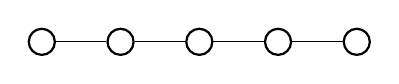
\begin{tikzpicture}[every node/.style={circle,thick,draw}]
  \node (1) {};
  \node (2) [ right of=1] {};
  \node (3) [ right of=2] {};
  \node (4) [ right of=3] {};
  \node (5) [ right of=4] {};
  \draw (1) -- (2);
  \draw (2) -- (3);
  \draw (3) -- (4);
  \draw (4) -- (5);
\end{tikzpicture}
\caption{Example of a small distributed network.}
\label{fig:dist_comp_1}
\end{figure}

According to Lamport \cite{DBLP:books/el/leeuwen90/LamportL90}, in the area of distributed computing, the term \emph{model} denotes a view or abstract representation of a distributed system.
There are multiple different computation models used in distributed computing.
The most important main category of distributed computation models is \emph{process models}.
In process models, the work or activities are represented as concurrently executed processes that execute their instructions sequentially.
The main way to distinguish different process models from each other is to categorise them by the method they use to communicate with each other (\emph{interprocess communication}).
\cite{DBLP:books/el/leeuwen90/LamportL90}


%\subsubsection{Message passing model} \label{sec:message_passing_model}
Message passing models are one form of a process model.
In the model, processes communicate by adding a message to a message queue, whether it is a shared or a process specific, and the recipient process moves the message out (dequeues) from the message queue.
\cite{DBLP:books/el/leeuwen90/LamportL90}

Different message passing models are widely used in the research field of distributed computing.
The models can varie in different details, such as in the size of the message queues \cite{DBLP:books/el/leeuwen90/LamportL90}, in the size of the messages \cite{peleg2000distributed} and on how the nodes get identified \cite{DBLP:conf/focs/Linial87}, if they are identified at all \cite{DBLP:conf/istcs/MayerNS95}.
%As the message passing models itself can be defined in multiple ways \cite{DBLP:books/el/leeuwen90/LamportL90}, we will use a definition from which the relevant models commonly inherit from.
We will dive deeper into the most relevant message passing models for this work in the following sections \ref{sec:port_number_model} and \ref{sec:local_model}.

An algorithm that is executed in a distributed fashion in a distributed network, is called as a distributed algorithm.
Each node in a network is started simultaneously and will always execute the same algorithm.
Initially the nodes are on the same state and there can be finitely or infinitely many states.
Initially the nodes are aware of only themselves and of the connections to their neighbours.
One might question that if every node starts with the same state, wouldn't they also end up in the same state?
Well yes, this happens inevitably in a case where the nodes were not given any additional symmetry breaking inputs and if every node sees the same amount of neighbours.
\cite{HirvonenSuomelaDistAlg2020}

%For example, we have a chain like network $W$ where each node $w$ has exactly two neighbours.
%The task is to execute an algorithm that finds the number of nodes in the network.


In practice, every computer node on a network has an UUID (Universally unique identifier) that can break the symmetry, and nodes are usually given some input data that they process, and nodes can always randomize data as they are never completely synchronized together, so this is not necessarily a problem.
In theory, we explicitly have to assume that there exists these kind of symmetry breaking elements.
In this works, distributed algorithms are deterministic unless otherwise mentioned.
In other research there might be randomizing involved.


\todo{Find a correct place to talk  about execution times if there is any}
In the message passing model, one could easily think that the execution time of the algorithm is the standard unit used to measure the performance but this is not true.
The message passing model implies that the dominant cost during an execution of a distributed algorithm is the message passing itself
\cite{DBLP:books/el/leeuwen90/LamportL90}.
This really... \todo{continue here}




%The following two sections (\ref{sec:port_number_model} and \ref{sec:local_model} ) talk about different forms of message passing models that are highly relative to this paper.

%In the theory of distributed computing, it is common to use terminology and concepts from graph theory as networks are basically graphs.
%With formal definitions, we can discuss more about the structure of distributed networks and reason features of those networks.
%We can further construct proofs of different theorems and so on. \todo{Fix this paragraph}

The algorithms that are executed in distributed fashion, are called distributed algorithms.
\todo{where to write about distributed algorithms?}
%A distributed algorithm is a specific type of algorithm that is executed in distributed fashion.
Specifically, each node executes the same algorithm.

%\todo{write about computation models, why they exist}


\subsubsection{Port number model} \label{sec:port_number_model}
This section is based on the course material from \cite{HirvonenSuomelaDistAlg2020} unless otherwise mentioned.

Port number model (PN model) is a rather weak model of computation that inherits from the message passing model.
In the model, nodes do not have identification.
An algorithm that executes in a port number model is called as a PN-algorithm.

We can basically take any network $N$ that has the same structure as a simple undirected graph $G$.
Each vertex of $G$ can be one-to-one mapped (bijection) to the nodes of $N$ and vice-versa.
Respectively all edges $\{v, w\}$ of $G$ can be mapped to communication channels between nodes $v$ and $w$.

Communication channels start and end from communication ports.
Each node has communication ports numbered from $1$ to $d$ where $d$ is the degree of the node.
The ports are numbered in an arbitrary order.

All nodes are considered identical, however nodes know their degree and it might differ between different nodes depending on the underlying graph $G$.
Every node starts the execution simultaneously following the same deterministic PN-algorithm $A$.
The execution of $A$ is done synchronously in parallel.
A communication round consists of following synchronous steps
\begin{enumerate}
  \item send message to each port,
  \item wait until all messages have been sent,
  \item receive a message from each port,
  \item update internal state.
\end{enumerate}
After each communication round, a node can optionally stop execution and announce its local output.
All nodes are required to eventually stop.
When all nodes have stopped, the algorithm is considered as stopped.
The running time of the algorithm $A$ is the total communication rounds that took place.








\subsubsection{Formalized port number model}
We call the network as a port number network or a PN-network
Port-numbering network is a 3-element tuple $N = (V, P, p)$, where V and P are the sets of vertices and ports respectively, and $p: P \rightarrow P$ is a function that maps a port to another port, forming a communication channel.
A port, an element of $P$, is a 2-element tuple $(v, i)$ where $v \in V$ and $i \in \{1, 2, ...\}$.
Additionally we assume that $p$ is an involution, that is, $\forall x \in P : p(p(x)) = x, $ i.e. each edge of the underlying graph is undirected.
See the figures \ref{fig:formal_pn1:a} and \ref{fig:formal_pn1:b} for examples of valid and invalid PN networks.

\begin{figure}[h]
  \subcaptionbox{A PN network of two nodes, $a$ and $b$.
    Both $a$ and $b$ have degree of 2, therefore 2 ports.
    Ports are $(a, 1), (a, 2), (b, 1)$ and $(b, 2)$.
    The connections are
      $p((a, 1)) = (b, 1)$,
      $p((a, 2)) = (b, 2)$,
      $p((b, 1)) = (a, 1)$ and
      $p((b, 2)) = (a, 2)$.
    \label{fig:formal_pn1:a}
  }%
    [.45\linewidth] {
    \centering
    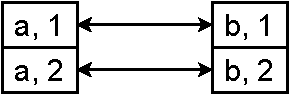
\includegraphics[scale=0.6]{diagrams/formalizing_pn_network_diagram1.pdf}
  }
  \hfill
  \subcaptionbox{
    An invalid PN network as port mapping function $p$ is not an involution:
    $p(p((a, 1))) = p(p((a, 2))) \neq (a, 1)$.
    \label{fig:formal_pn1:b}
  }%
    [.45\linewidth] {
    \centering
    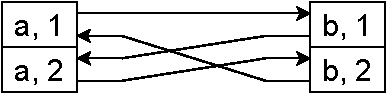
\includegraphics[scale=0.6]{diagrams/formalizing_pn_network_diagram2.pdf}
  }
  \caption{Examples of a valid and an invalid PN network.}
  \label{fig:formal_pn1}
\end{figure}


\begin{figure}[h]
  \subcaptionbox{
    A simple PN network.
    The underlying graph is also simple.
    \label{fig:formal_pn2:a}
  }%
    [.3\linewidth] {
    \centering
    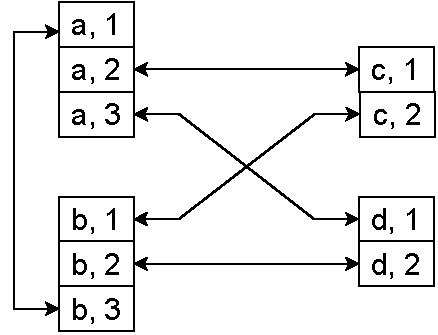
\includegraphics[scale=0.6]{diagrams/formalizing_pn_network_diagram4.pdf}
  }
  \hfill
  \subcaptionbox{
    An alternative representation of the PN network from figure \ref{fig:formal_pn2:b}
    \label{fig:formal_pn2:b}
  }%
    [.3\linewidth] {
    \centering
    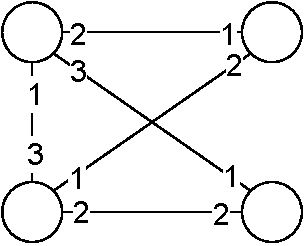
\includegraphics[width=0.3\textwidth]{diagrams/formalizing_pn_network_diagram5.pdf}
  }
  \hfill
  \subcaptionbox{
    A PN network with loops and parallel connections.
    This kind of network cannot be shown in the alternative representation unlike the network on figure \ref{fig:formal_pn2:a}.
    \label{fig:formal_pn2:c}
  }%
    [.3\linewidth] {
    \centering
    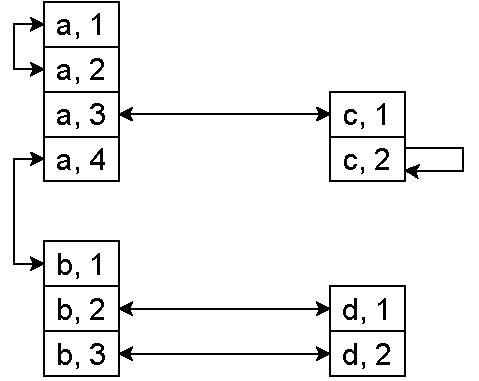
\includegraphics[scale=0.6]{diagrams/formalizing_pn_network_diagram3.pdf}
  }
  \caption{Examples of simple and non simple PN networks.}
  \label{fig:formal_pn2}
\end{figure}

\todo{continue from here on  FRIDAY 31.12.2021}
Each node is able to index their neighbour nodes using port numbers.
Port numbers range from 1 to d where d is the degree of the node.

Computation in a distributed network happens in synchronized rounds.
In the previous section \ref{sec:port_number_model} we introduced the PN model.
Now we give a formal definition of the PN model.


\todo{Add formal definition here}
Port numbering algorithm is ...



\subsubsection{LOCAL model} \label{sec:local_model}

\subsection{LCL problems} \label{sec:lcl_problems}

\subsection{Boolean satisfiability problem}

\subsection{Previous research} \label{sec:previous_research}

\todo{Especially LCL classification research}

\clearpage

